\begin{figure}[htbp]
\centering
\resizebox{\textwidth}{!}{%
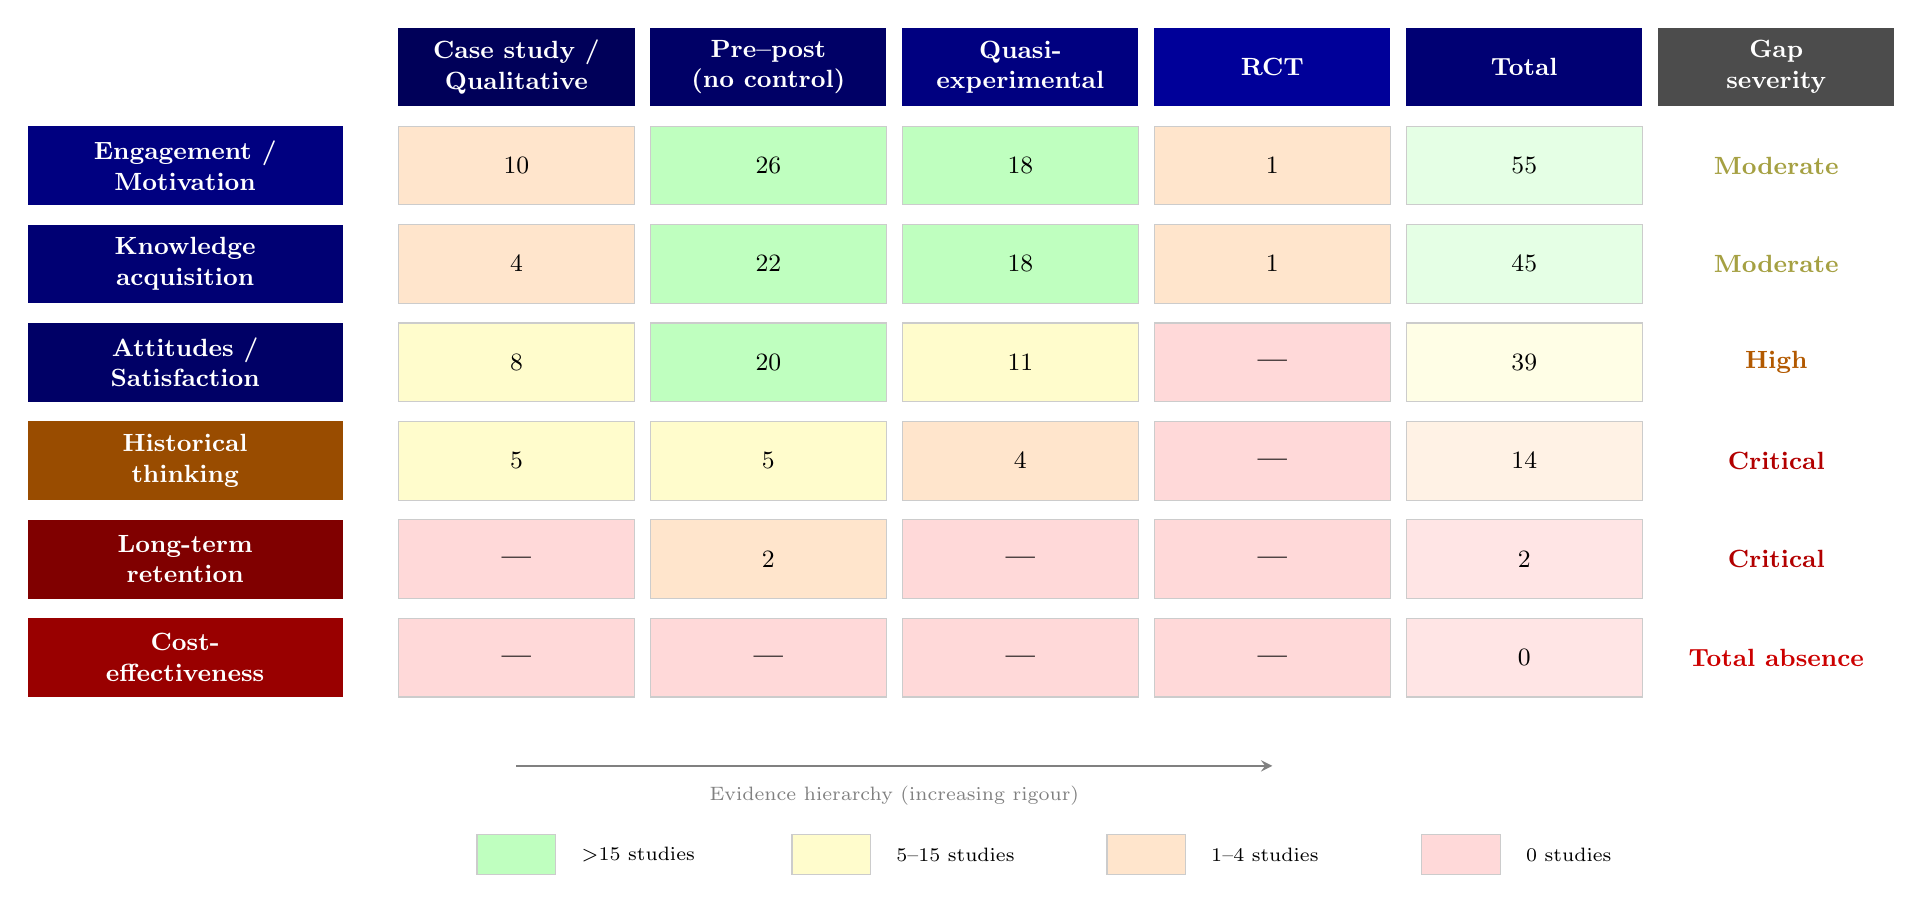
\begin{tikzpicture}[
  hdr/.style={font=\small\bfseries, text=white, minimum height=1.0cm,
    minimum width=3.0cm, align=center},
  rhdr/.style={font=\small\bfseries, text=white, minimum height=1.0cm,
    minimum width=4.0cm, align=center, anchor=east},
  cell/.style={rectangle, draw=gray!40, minimum height=1.0cm,
    minimum width=3.0cm, align=center, font=\small},
  dense/.style={cell, fill=green!25},
  moderate/.style={cell, fill=yellow!20},
  sparse/.style={cell, fill=orange!20},
  empty/.style={cell, fill=red!15, font=\small\bfseries},
  gap/.style={font=\small\bfseries, minimum height=1.0cm,
    minimum width=3.2cm, align=center},
]

% Column spacing
\def\colw{3.2}

% Column headers
\node[hdr, fill=blue!35!black] at (0, 0) {Case study /\\Qualitative};
\node[hdr, fill=blue!40!black] at (\colw, 0) {Pre--post\\(no control)};
\node[hdr, fill=blue!50!black] at (2*\colw, 0) {Quasi-\\experimental};
\node[hdr, fill=blue!60!black] at (3*\colw, 0) {RCT};
\node[hdr, fill=blue!45!black] at (4*\colw, 0) {Total};
\node[hdr, fill=gray!60!black] at (5*\colw, 0) {Gap\\severity};

% Row spacing
\def\rowh{1.25}

% Row 1: Engagement / Motivation
\node[rhdr, fill=blue!50!black] at (-2.2, -\rowh) {Engagement /\\Motivation};
\node[sparse] at (0, -\rowh) {10};
\node[dense] at (\colw, -\rowh) {26};
\node[dense] at (2*\colw, -\rowh) {18};
\node[sparse] at (3*\colw, -\rowh) {1};
\node[cell, fill=green!10] at (4*\colw, -\rowh) {55};
\node[gap, text=yellow!60!black] at (5*\colw, -\rowh) {Moderate};

% Row 2: Knowledge acquisition
\node[rhdr, fill=blue!45!black] at (-2.2, -2*\rowh) {Knowledge\\acquisition};
\node[sparse] at (0, -2*\rowh) {4};
\node[dense] at (\colw, -2*\rowh) {22};
\node[dense] at (2*\colw, -2*\rowh) {18};
\node[sparse] at (3*\colw, -2*\rowh) {1};
\node[cell, fill=green!10] at (4*\colw, -2*\rowh) {45};
\node[gap, text=yellow!60!black] at (5*\colw, -2*\rowh) {Moderate};

% Row 3: Attitudes / Satisfaction
\node[rhdr, fill=blue!40!black] at (-2.2, -3*\rowh) {Attitudes /\\Satisfaction};
\node[moderate] at (0, -3*\rowh) {8};
\node[dense] at (\colw, -3*\rowh) {20};
\node[moderate] at (2*\colw, -3*\rowh) {11};
\node[empty] at (3*\colw, -3*\rowh) {---};
\node[cell, fill=yellow!10] at (4*\colw, -3*\rowh) {39};
\node[gap, text=orange!70!black] at (5*\colw, -3*\rowh) {High};

% Row 4: Historical thinking
\node[rhdr, fill=orange!60!black] at (-2.2, -4*\rowh) {Historical\\thinking};
\node[moderate] at (0, -4*\rowh) {5};
\node[moderate] at (\colw, -4*\rowh) {5};
\node[sparse] at (2*\colw, -4*\rowh) {4};
\node[empty] at (3*\colw, -4*\rowh) {---};
\node[cell, fill=orange!10] at (4*\colw, -4*\rowh) {14};
\node[gap, text=red!70!black] at (5*\colw, -4*\rowh) {Critical};

% Row 5: Long-term retention
\node[rhdr, fill=red!50!black] at (-2.2, -5*\rowh) {Long-term\\retention};
\node[empty] at (0, -5*\rowh) {---};
\node[sparse] at (\colw, -5*\rowh) {2};
\node[empty] at (2*\colw, -5*\rowh) {---};
\node[empty] at (3*\colw, -5*\rowh) {---};
\node[cell, fill=red!10] at (4*\colw, -5*\rowh) {2};
\node[gap, text=red!70!black] at (5*\colw, -5*\rowh) {Critical};

% Row 6: Cost-effectiveness
\node[rhdr, fill=red!60!black] at (-2.2, -6*\rowh) {Cost-\\effectiveness};
\node[empty] at (0, -6*\rowh) {---};
\node[empty] at (\colw, -6*\rowh) {---};
\node[empty] at (2*\colw, -6*\rowh) {---};
\node[empty] at (3*\colw, -6*\rowh) {---};
\node[cell, fill=red!10] at (4*\colw, -6*\rowh) {0};
\node[gap, text=red!80!black] at (5*\colw, -6*\rowh) {Total absence};

% Bottom annotation: evidence hierarchy arrow
\draw[-stealth, thick, black!50] (0, -7.1*\rowh) -- (3*\colw, -7.1*\rowh);
\node[font=\scriptsize, text=black!50, anchor=north] at (1.5*\colw, -7.2*\rowh)
    {Evidence hierarchy (increasing rigour)};

% Legend
\node[dense, minimum width=1.0cm, minimum height=0.5cm] at (0, -8*\rowh) {};
\node[font=\scriptsize, anchor=west] at (0.7, -8*\rowh) {$>$15 studies};
\node[moderate, minimum width=1.0cm, minimum height=0.5cm] at (4.0, -8*\rowh) {};
\node[font=\scriptsize, anchor=west] at (4.7, -8*\rowh) {5--15 studies};
\node[sparse, minimum width=1.0cm, minimum height=0.5cm] at (8.0, -8*\rowh) {};
\node[font=\scriptsize, anchor=west] at (8.7, -8*\rowh) {1--4 studies};
\node[empty, minimum width=1.0cm, minimum height=0.5cm] at (12.0, -8*\rowh) {};
\node[font=\scriptsize, anchor=west] at (12.7, -8*\rowh) {0 studies};

\end{tikzpicture}%
}% end resizebox
\caption{Evidence gap map for gamification in history education. Rows represent outcome domains; columns represent study design types ordered by evidence hierarchy. Cell values indicate the number of studies; colour intensity indicates evidence density. Critical gaps in historical thinking, long-term retention, and cost-effectiveness represent priority targets for future research. No outcome domain has evidence from adequately powered RCTs.}
\label{fig:evidence-gap-map}
\end{figure}
